\section{Motivation: Ill-posed inverse problems}

Inverse problems consist of retrieving the information about the states of a given system by means of (incomplete) observations.
Such problems can be cast into the following measurement (observation) equation
\begin{equation}
    \label{eq:measurement_equation}
    Y = f(\state, Z) \eqsp.
\end{equation}
We call $Y$ the observation variable, $\state$ the state variable, $Z$ the noise variable and $f$ the measurement function.
In inverse problems, we have a realization $y \sim Y$ and we want to say which are the states $X$ that can be "associated" to $y$.

\paragraph{Linear inverse problems}

The most simple case we can imagine is a linear inverse problem with Gaussian noise, 
\begin{equation*}
    Y = A \state + \sigma_y Z \eqsp,
\end{equation*}
where $A \in \mxset{d_y}{\statedim}$, $Z \sim \gauss(0, \idm_{d_y})$ and $\sigma_y > 0$. This can be seen as a linear regression problem, but while
linear regression deals mostly with the case $d_y > \statedim$, in inverse problems we are interested in the case $d_y \ll \statedim$.
Before going further into solving inverse problems, let's see some examples.

\paragraph{Inpainting on images}

The most visual example is the case of inpainting. Suppose we have only observed a part of an image, and we want to reconstruct the whole image, as shown in \cref{fig:inpainting_example}
\begin{figure}[h!]
    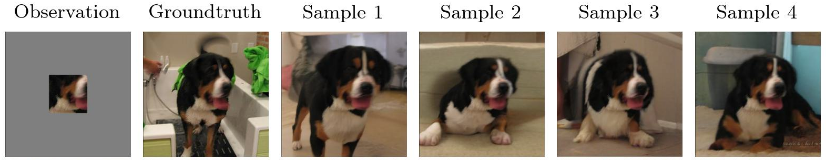
\includegraphics[width=\textwidth]{images_gabriel/example_inpainting_yazid.png}
    \label{fig:inpainting_example}
    \caption{Figure taken from \cite{moufad2024variational}. The "Observation" corresponds to $y$ that was obtained with the ground truth $\state$. The other columns correspond to solutions of a certain inverse problem.}
\end{figure}
In this case, we can see that the matrix $A$ is a diagonal (if we "flatten" the image vector) matrix with $0$ corresponding to the unobserved pixels and $1$ on the observed pixels.

\paragraph{Recovering the soil profiles from drill measurements}

In \cite{bhavsar2023principled}, the authors proposed a solution to the inpainting problems where the state is a 3d volume corresponding to the different layers that constitute the soil 
from drill measurements (vertical wells were drilled and the soil composition was measured along the drill) as shown in \cref{fig:flummy_example}

\begin{figure}[h!]
    \centering
    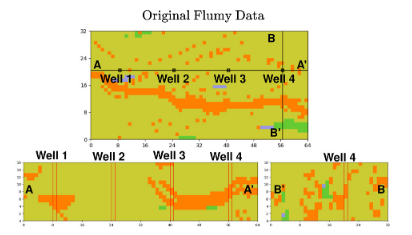
\includegraphics[width=0.6\textwidth]{images_gabriel/example_flummy.png}
    \label{fig:flummy_example}
    \caption{Figure taken from \cite{bhavsar2023principled}.}
\end{figure}

\paragraph{Non-diagonal linear problems}
While we have for the moment focused on rather simple $A$, there can be much more complicated $A$, such as Gaussian debluring, motion bluring, super resolution...

\subsection{Statistical formulation: What do we want?}

\paragraph{Context:}
Let's focus on the soil profiles problem. You are an environmental agent and you should decide to authorize or not the drilling in a certain region.
You have to determine if the drilling of the region affects the water resources of the region.
The only information you have is the drilling profiles for certain wells, as in \cref{fig:flummy_example}, which we denote by $y$.
Let denote by $A$ the event corresponding to the fact that there is an underground channel passing through $A$.

A decision problem corresponds of a tuple $(\stateset, \rewardset, \actionset, U)$, where
\begin{itemize}
    \item $\stateset$ is the set of states of the world: For us, the whole profile of the soil in the whole region and our measurements, denoted by $(\state, Y)$ and that we assume that lives in $\rset^{\statedim} \times \rset^{d_y}$.
    \item $\rewardset$ is the set of reward, which I propose that we model as $\{0, 1\}^2$, which corresponds to answer to two questions: "Do I think there is water in A?" and "Is there water in A?"
    \item $\actionset$ is the action space, which are functions $a: \stateset \rightarrow \rewardset$ that we impose to be of the form $a(\lstate, y) = (g(y), \indi{A}(\lstate))$ where $g: \rset^{d_y} \rightarrow \{0, 1\}$.
    \item $U: \rewardset \rightarrow \rset$ is the utility function. It is often useful to consider it as matrix $\m{U} \in \mxset{2}{2}$ such that $U(z_1, z_2) = (z_1, 1 - z_1)^t \m{U} (z_2, 1 - z_2)$.
\end{itemize}
Our goal is of course to obtain the solution that maximizes the utility in some sense, but of course we don't know a part of the state (at least before authorizing or not the drilling).
The definition of the way we maximize utility is the frontier between frequentists and Bayesian. In our case though, simply maximizing $U(a(x, y))$ over the whole space has of course no point!

\paragraph{Wait, why can't we simply maximize the likelihood?}

Note that the likelihood depends only on the values of $\state$ in the drilled wells. So anything else in the rest of the domain is Ok!

\paragraph{Maximizing Subjective expected utility}

Bayesian statisticians such as DeFinetti and Savage propose to solve subjective expected utility (SEU) problem
\begin{equation}
    \argmax_{a \in \mathcal{A}} \PE{\tilde{p}}{U(a(\state, Y))} \eqsp,
\end{equation}
where $\tilde{p}(\lstate, y) = p(\lstate) \gauss(y; \m{A}x, \sigma_y^2 \idm)$ and $p$ is a prior (subjective) distribution over the unobserved states.

Note that we have $\PE{\tilde{p}}{U(a(\state, Y))} = \sum_{(i, j) \in \{0, 1\}^2} u_{i, j} \PE{\tilde{p}}{g(Y)^{i}(1 - g(Y))^{1-i}(1 - \indi{A}(X))^{1-j}\indi{A}(X)^j}$.
and that typically we would have $u_{i, j} \leq 0$ if $i != j$ and $u_{i, i} > 0$.
Convince yourself that we want to study the following quantity 
\[
    \PE{\tilde{p}}{g(Y) \indi{A}(\state)} \eqsp.
\]  
By Bayes rule
\[
    \PE{\tilde{p}}{g(Y) \indi{A}(\state)} = \PE{p_y}{g(Y) \PE{\ppostd{\cdot}[y=Y]}{\indi{A}(\state)}} \eqsp,
\] 
where $p_y(y) = \int \gauss(y, \m{A}\lstate, \sigma_y^2 \idm) p(\rmd \lstate)$ and $\ppostd{\lstate} =  p(\lstate) \gauss(y; \m{A}x, \sigma_y^2 \idm) / p_y(y)$.

The Bayes action is the action associated with $g$ that maximizes
\begin{equation}
    \label{eq:bayes_action}
    g(Y) \PE{\ppostd{\cdot}[y=Y]}{\indi{A}(\state)}    
\end{equation}
almost surely with respect to $p_y$. This is the kind of action that we must look and therefore it is \textbf{key to known the posterior $\ppost$}.

\paragraph{How do we define the prior $p(\lstate)$?}

There are several ways to define a prior over the space of states. Traditionally, we would penalize the states (L$2$ regularization) or impose the solution to be the outcome
of a simulation and reduce the dimensionality to a set of simulation's parameters.

Recently, with the increase availability of data, generative models \textbf{provide a way to build priors relying only on observed data}.
This is particularly interesting in high dimensional complicated datasets such as image, audio and video, where prior to this no realistic model existed.
In this notes we investigate how to approximate the posterior of such priors.

\subsection{Latent model priors}

In this section we investigate general methodology to treat priors issued from latent models, namely VAEs and GANs.

\subsection{Denoising diffusion priors}

To be written